
\documentclass[border=10pt, 12pt]{standalone}
\usepackage[svgnames]{xcolor}
\usepackage{amsmath}
\usepackage{pgfplots}
\pgfplotsset{compat=newest}
\usepackage[sfdefault]{FiraSans}
\usepackage{FiraMono}
\renewcommand*\familydefault{\sfdefault}
\begin{document}
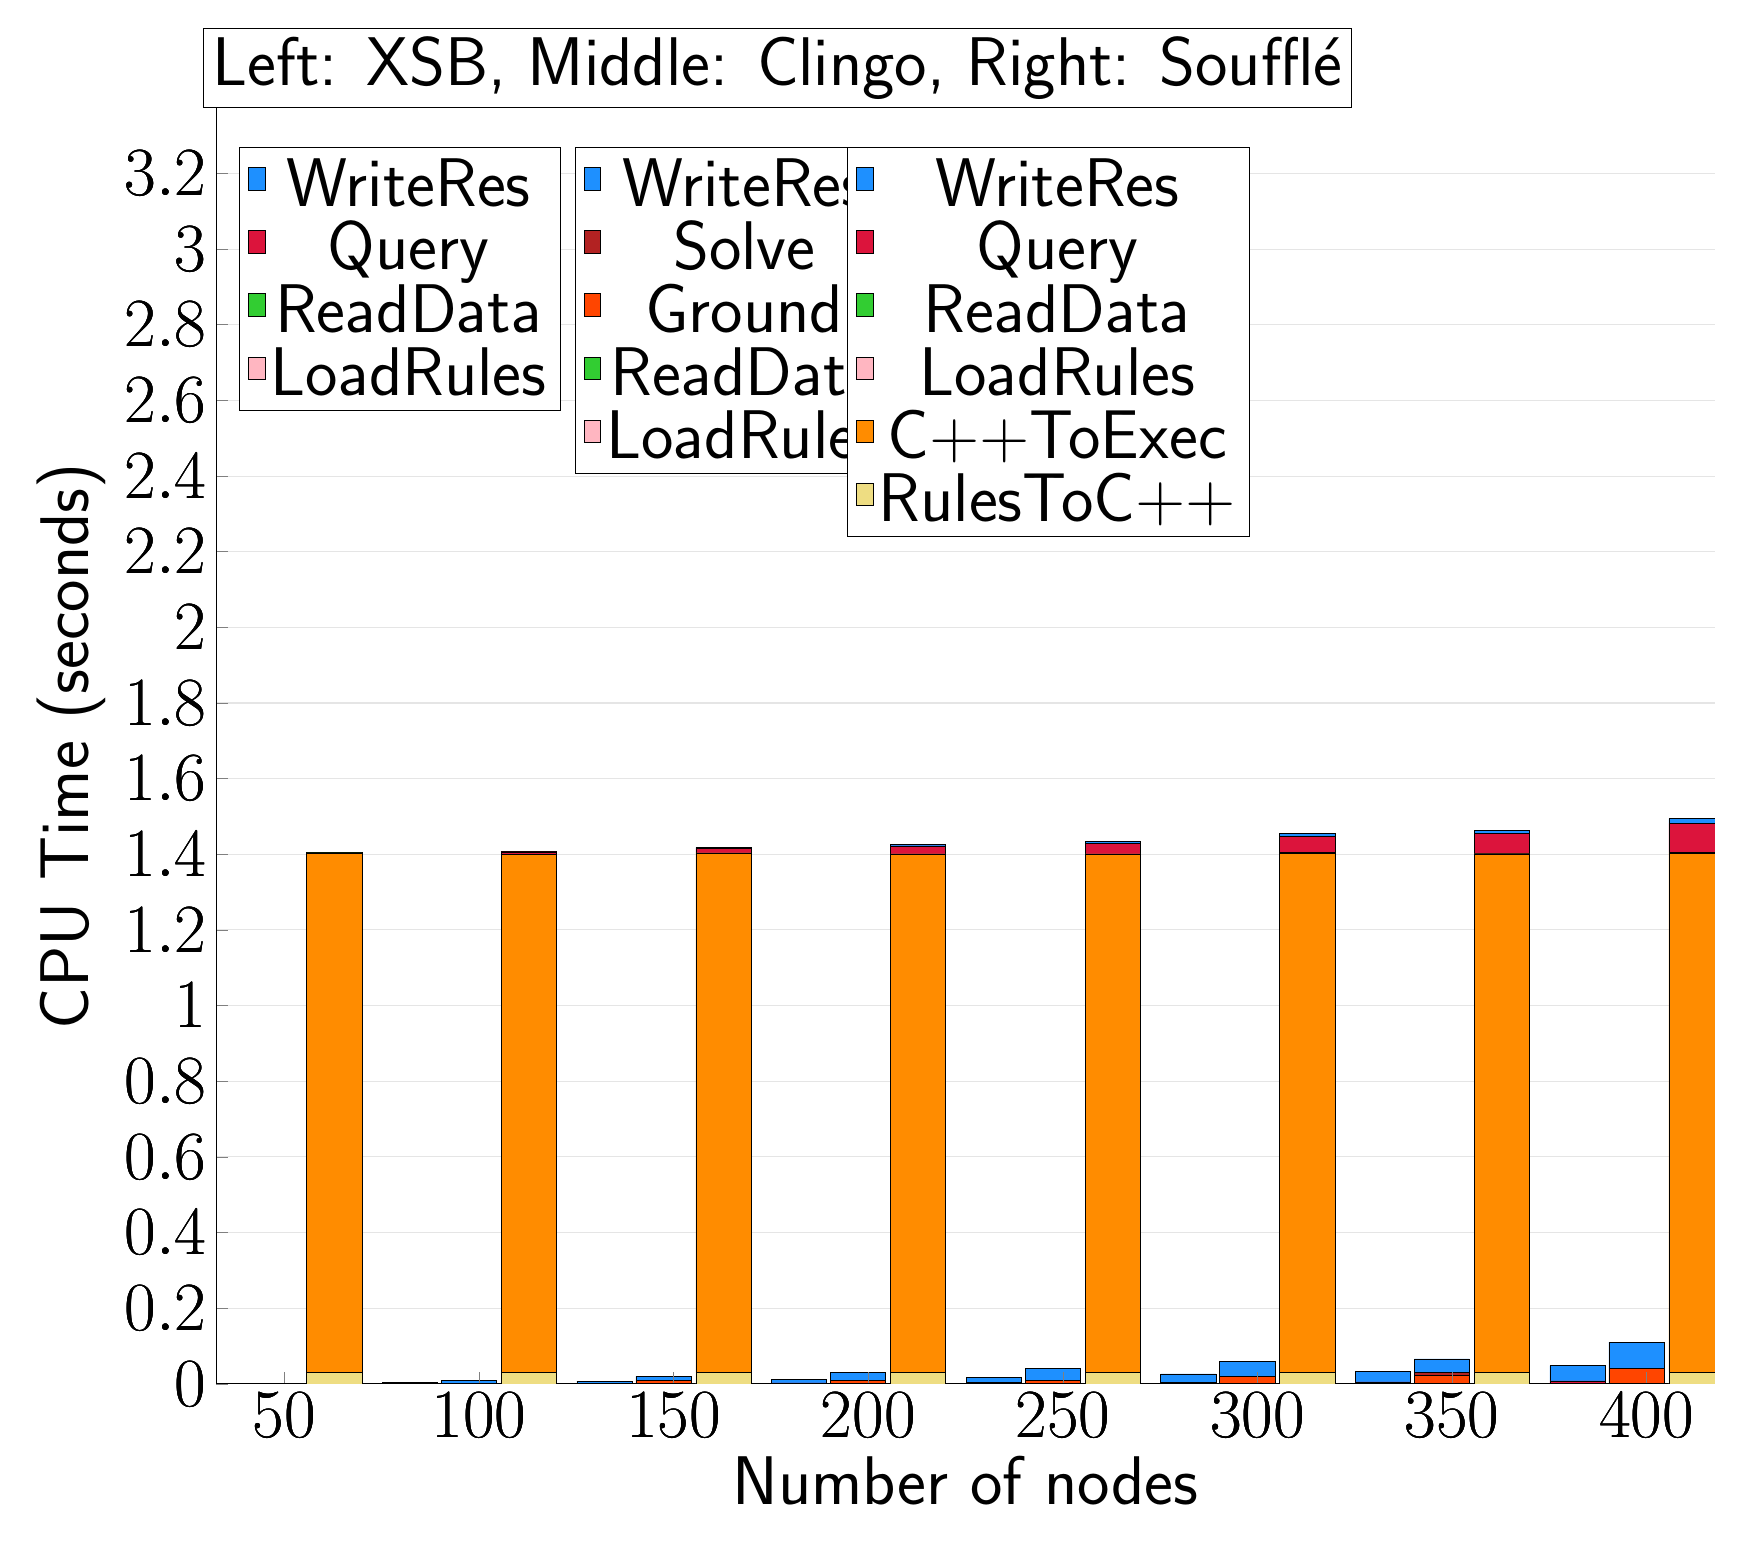
\begin{tikzpicture}
	\begin{axis}[bar shift=-25pt,
			ybar stacked,
			width=1.7\textwidth,
			bar width=0.7cm,
			ymajorgrids, tick align=inside,
			major grid style={draw=gray!20},
			xtick=data,
			ymin=0, ymax=3.3720000000000003,
			axis x line*=bottom,
			axis y line*=left,
			enlarge x limits=0.05,
			legend style={
					at={(0.23, 0.97)},
					anchor=north east,
					legend columns=1,
					font=\Huge,
				},
			ylabel={CPU Time (seconds)},
			xlabel={Number of nodes},
			label style={font=\Huge},
			tick label style={font=\Huge},
		]
		\addlegendimage{fill=DodgerBlue, draw=black, line width=0.2pt}
		\addlegendentry{WriteRes}
		\addlegendimage{fill=Crimson, draw=black, line width=0.2pt}
		\addlegendentry{Query}
		\addlegendimage{fill=LimeGreen, draw=black, line width=0.2pt}
		\addlegendentry{ReadData}
		\addlegendimage{fill=LightPink, draw=black, line width=0.2pt}
		\addlegendentry{LoadRules}
		\addplot +[fill=LightPink, draw=black, line width=0.2pt] coordinates {
				(50, 0.0006234)
				(100, 0.0006140000000000003)
				(150, 0.0005979000000000003)
				(200, 0.0006039000000000003)
				(250, 0.0006099000000000002)
				(300, 0.0006162999999999999)
				(350, 0.0006065000000000005)
				(400, 0.0006103999999999998)
			};
		\addplot +[fill=LimeGreen, draw=black, line width=0.2pt] coordinates {
				(50, 0.0002159999999999999)
				(100, 0.00028549999999999973)
				(150, 0.00035489999999999995)
				(200, 0.0004419999999999997)
				(250, 0.0004924999999999992)
				(300, 0.0006106999999999998)
				(350, 0.0006636000000000005)
				(400, 0.0007914000000000008)
			};
		\addplot +[fill=Crimson, draw=black, line width=0.2pt] coordinates {
				(50, 0.00011319999999999969)
				(100, 0.0004071)
				(150, 0.0008225000000000003)
				(200, 0.0015279)
				(250, 0.002016)
				(300, 0.0032730000000000003)
				(350, 0.0039008000000000003)
				(400, 0.0065328999999999995)
			};
		\addplot +[fill=DodgerBlue, draw=black, line width=0.2pt] coordinates {
				(50, 0.0007389999999999999)
				(100, 0.0026892)
				(150, 0.0055813)
				(200, 0.0100794)
				(250, 0.013255799999999998)
				(300, 0.021685199999999998)
				(350, 0.0267913)
				(400, 0.0402019)
			};
	\end{axis}

	\begin{axis}[bar shift=-3.7pt,
			ybar stacked,
			width=1.7\textwidth,
			bar width=0.7cm,
			ymajorgrids, tick align=inside,
			major grid style={draw=none},
			xtick=data,
			ymin=0, ymax=3.3720000000000003,
			axis x line*=none,
			axis y line*=none,
			enlarge x limits=0.05,
			legend style={
					at={(0.454, 0.97)},
					anchor=north east,
					legend columns=1,
					font=\Huge,
				},
			label style={font=\Huge},
			tick label style={font=\Huge},
		]
		\addlegendimage{fill=DodgerBlue, draw=black, line width=0.2pt}
		\addlegendentry{WriteRes}
		\addlegendimage{fill=FireBrick, draw=black, line width=0.2pt}
		\addlegendentry{Solve}
		\addlegendimage{fill=OrangeRed, draw=black, line width=0.2pt}
		\addlegendentry{Ground}
		\addlegendimage{fill=LimeGreen, draw=black, line width=0.2pt}
		\addlegendentry{ReadData}
		\addlegendimage{fill=LightPink, draw=black, line width=0.2pt}
		\addlegendentry{LoadRules}
		\addplot +[fill=LightPink, draw=black, line width=0.2pt] coordinates {
				(50, 0.0)
				(100, 0.0)
				(150, 0.0)
				(200, 0.0)
				(250, 0.0)
				(300, 0.0)
				(350, 0.0)
				(400, 0.0)
			};
		\addplot +[fill=LimeGreen, draw=black, line width=0.2pt] coordinates {
				(50, 0.0)
				(100, 0.0)
				(150, 0.0)
				(200, 0.0)
				(250, 0.0)
				(300, 0.0)
				(350, 0.0)
				(400, 0.0)
			};
		\addplot +[fill=OrangeRed, draw=black, line width=0.2pt] coordinates {
				(50, 0.0)
				(100, 0.0)
				(150, 0.009999999999999997)
				(200, 0.009999999999999997)
				(250, 0.009999999999999997)
				(300, 0.019999999999999997)
				(350, 0.023)
				(400, 0.03999999999999999)
			};
		\addplot +[fill=FireBrick, draw=black, line width=0.2pt] coordinates {
				(50, 0.0)
				(100, 0.0)
				(150, 0.0)
				(200, 0.0)
				(250, 0.0)
				(300, 0.0)
				(350, 0.007000000000000001)
				(400, 0.0)
			};
		\addplot +[fill=DodgerBlue, draw=black, line width=0.2pt] coordinates {
				(50, 0.0)
				(100, 0.009999999999999997)
				(150, 0.010000000000000004)
				(200, 0.020000000000000007)
				(250, 0.030000000000000006)
				(300, 0.039999999999999994)
				(350, 0.03599999999999999)
				(400, 0.07000000000000002)
			};
	\end{axis}

	\begin{axis}[bar shift=18pt,
			ybar stacked,
			width=1.7\textwidth,
			bar width=0.7cm,
			ymajorgrids, tick align=inside,
			major grid style={draw=none},
			xtick=data,
			ymin=0, ymax=3.3720000000000003,
			axis x line*=none,
			axis y line*=none,
			enlarge x limits=0.05,
			legend style={
					at={(0.69, 0.97)},
					anchor=north east,
					legend columns=1,
					font=\Huge,
				},
			label style={font=\Huge},
			tick label style={font=\Huge},
		]
		\addlegendimage{fill=DodgerBlue, draw=black, line width=0.2pt}
		\addlegendentry{WriteRes}
		\addlegendimage{fill=Crimson, draw=black, line width=0.2pt}
		\addlegendentry{Query}
		\addlegendimage{fill=LimeGreen, draw=black, line width=0.2pt}
		\addlegendentry{ReadData}
		\addlegendimage{fill=LightPink, draw=black, line width=0.2pt}
		\addlegendentry{LoadRules}
		\addlegendimage{fill=DarkOrange, draw=black, line width=0.2pt}
		\addlegendentry{C++ToExec}
		\addlegendimage{fill=LightGoldenrod, draw=black, line width=0.2pt}
		\addlegendentry{RulesToC++}
		\addplot +[fill=LightGoldenrod, draw=black, line width=0.2pt] coordinates {
				(50, 0.030000000000000006)
				(100, 0.030000000000000006)
				(150, 0.030000000000000006)
				(200, 0.030000000000000006)
				(250, 0.030000000000000006)
				(300, 0.030000000000000006)
				(350, 0.030000000000000006)
				(400, 0.030000000000000006)
			};
		\addplot +[fill=DarkOrange, draw=black, line width=0.2pt] coordinates {
				(50, 1.3730000000000002)
				(100, 1.3700000000000003)
				(150, 1.3730000000000004)
				(200, 1.3700000000000003)
				(250, 1.3700000000000003)
				(300, 1.3730000000000004)
				(350, 1.371)
				(400, 1.373)
			};
		\addplot +[fill=LightPink, draw=black, line width=0.2pt] coordinates {
				(50, 0.0001155)
				(100, 0.0001163)
				(150, 9.919999999999999e-05)
				(200, 9.95e-05)
				(250, 0.00011270000000000002)
				(300, 0.00011279999999999999)
				(350, 0.00010870000000000001)
				(400, 9.2e-05)
			};
		\addplot +[fill=LimeGreen, draw=black, line width=0.2pt] coordinates {
				(50, 0.0004068)
				(100, 0.0006006)
				(150, 0.0007356999999999999)
				(200, 0.000959)
				(250, 0.0010628999999999999)
				(300, 0.0013739000000000002)
				(350, 0.0014149)
				(400, 0.0017656999999999998)
			};
		\addplot +[fill=Crimson, draw=black, line width=0.2pt] coordinates {
				(50, 0.0012343)
				(100, 0.005648200000000001)
				(150, 0.0114977)
				(200, 0.0213543)
				(250, 0.027607100000000002)
				(300, 0.0431208)
				(350, 0.051973300000000014)
				(400, 0.0771452)
			};
		\addplot +[fill=DodgerBlue, draw=black, line width=0.2pt] coordinates {
				(50, 0.0005489000000000001)
				(100, 0.0015336)
				(150, 0.0027530999999999996)
				(200, 0.0042326)
				(250, 0.005171)
				(300, 0.0073131)
				(350, 0.0086033)
				(400, 0.012383700000000001)
			};
	\end{axis}


	\node[anchor=south, draw, fill=white] at (rel axis cs:0.42,1) {\Huge Left: XSB, Middle: Clingo, Right: Soufflé};
\end{tikzpicture}
\end{document}
